

% Perspectives for HET physics studies at a muon-hadron collider at CERN
% HELP4CERN Study Group
% DIS 2026, 4-8 May 2026, Bologna, Italy


\documentclass[a4paper,11pt]{article}

\usepackage{pos}
\usepackage{amsmath}
\usepackage{booktabs}
\usepackage{tabularx}

\usepackage{ragged2e}
\usepackage{etoolbox}

\usepackage{tikz}
\usepackage{comment}

\usepackage{tikz-feynman}
\tikzfeynmanset{compat=1.1.0}

\usetikzlibrary{calc,positioning,arrows.meta,decorations.pathmorphing,patterns,shapes.geometric}

\usepackage{hyperref}

\usepackage[table]{xcolor}

\newcommand{\lhmuc}{LH$\mu$C}
\newcommand{\Lumi}{\mathcal{L}_{\mathrm{int}}}
\newcommand{\BR}{\mathrm{BR}}
\newif\ifPhotonFigure
\PhotonFiguretrue


\title{Perspectives for HET physics studies at a muon-hadron collider at CERN}
\ShortTitle{HET physics at a muon-hadron collider at CERN}
\author*[a]{Hamzeh Khanpour}
\onbehalf*{(on behalf of HELP4CERN Study Group)}
\affiliation[a]{AGH University of Krakow, Faculty of Physics and Applied Computer Science,
Al. Mickiewicza 30, 30-055 Krak\'ow, Poland.}
\emailAdd{hamzeh.khanpour@cern.ch} 


%-----------------------------------
\abstract{%
A muon-hadron collider at CERN would combine the energy reach of a 
TeV-scale muon beam with the proton beam of the High-Luminosity LHC, opening 
a programme of Higgs, electroweak and top (HET) studies. 
We discuss the HELP4CERN prospects for muon energies of 0.5, 1 and 2~TeV, corresponding to centre-of-mass 
energies of approximately 3.74, 5.3 and 7.5~TeV for 7~TeV protons. 
The accessible deep-inelastic-scattering (DIS) phase space and inclusive production 
rates provide the basis for the physics programme. Particular attention is given to a 
dedicated charged-current $h\to b\bar b$ study and an exploratory combined Higgs-coupling fit, 
distinguishing statistical rate precision from coupling constraints that depend on external information 
and fit assumptions. Electroweak and top measurements, photon-induced production, and muon-coupled new-physics 
channels offer complementary directions. }
%-----------------------------------


\FullConference{33rd International Workshop on Deep Inelastic Scattering and Related Subjects (DIS2026)\\
4-8 May 2026, Bologna, Italy} 





\begin{document}
\maketitle



%===============================
\section{Collider benchmarks and HET production rates}\label{sec:setup}
%===============================


The proposed \lhmuc\ would collide a positive-muon beam with the 7~TeV proton beam of the 
High-Luminosity LHC, extending the lepton-hadron programme beyond the electron-beam 
configurations of the LHeC~\cite{Akturk:2025ubm,LHeC:2020van,Ahmadova:2025vzd}. This contribution focuses on 
the Higgs, electroweak and top (HET) programme, complemented by photon-induced reactions and 
selected new-physics opportunities~\cite{Khanpour:DIS2026,HELP4CERN}. 
The inclusive production cross-sections for the Higgs and top-quark are reported in Table~\ref{tab:rates}. 
The large charged-current (CC) and neutral-current (NC) Higgs samples and the increasing single-top and top-pair 
rates motivate detailed measurements.  

%-----------------------------------------
\begin{table}[htbp]
\centering
\small
\setlength{\tabcolsep}{6pt}
\renewcommand{\arraystretch}{1.18}
\begin{tabular}{lcccc}
\toprule
Process & 20~GeV & 50~GeV & 500~GeV & 1~TeV\\
& LHeC   & LHeC   & \lhmuc  & \lhmuc\\
\midrule
$\sigma(\ell p\to\nu_\ell H+\mathrm{jet}+X)$ [fb]
& 52 & 164 & 438 & 731 \\
		
$\sigma(\ell p\to\ell H+\mathrm{jet}+X)$ [fb]
& 5.6 & 19 & 135 & 221 \\
		
$\sigma(\ell p\to\ell t\bar t+X)$ [pb]
& 0.0015 & 0.0323 & 1.03 & 2.23 \\
		
$\sigma(\ell p\to\nu_\ell t+X)$ [pb]
& 0.55 & 2.89 & 21.26 & 36.77 \\
\bottomrule
\end{tabular}
\caption{Benchmark inclusive production cross-sections for
Higgs-boson, top-quark-pair, and single-top production at the
LHeC and \lhmuc. 
In the LHeC cases an 80\% electron beam polarisation is assumed~\cite{Andre:2025iar}.}
\label{tab:rates}
\end{table}
%-----------------------------------------

The \lhmuc\ working points are summarized in Table~\ref{tab:benchmarks}. 
The first option employs a 500~GeV muon beam, 
giving a centre-of-mass energy of approximately 3.7~TeV and a projected
integrated luminosity of $250~\mathrm{fb}^{-1}$. The nominal baseline
uses a 1~TeV muon beam, corresponding to $\sqrt{s_{\mu p}}\simeq5.3$~TeV,
with a benchmark integrated luminosity of $1000~\mathrm{fb}^{-1}$. 
The second option increases the muon-beam energy to 2~TeV, reaching
$\sqrt{s_{\mu p}}\simeq7.5$~TeV with the same benchmark integrated
luminosity. 

%-----------------------------------------
\begin{table}[htbp]
\centering
\small
\setlength{\tabcolsep}{6pt}
\renewcommand{\arraystretch}{1.18}
\begin{tabular}{lcccc}
\toprule
Configuration
& $E_\mu$
& $E_p$
& $\sqrt{s_{\mu p}}$
& $\mathcal{L}_{\mathrm{int}}$\\
\midrule
First option
& 500~GeV & 7~TeV & 3.7~TeV
& $250~\mathrm{fb}^{-1}$\\
		
Nominal baseline
& 1~TeV & 7~TeV & 5.3~TeV
& $1000~\mathrm{fb}^{-1}$\\
		
Second option
& 2~TeV & 7~TeV & 7.5~TeV
& $1000~\mathrm{fb}^{-1}$\\
\bottomrule
\end{tabular}
\caption{Benchmark \lhmuc\ working points based on the HELP4CERN
studies~\cite{HELP4CERN}. The integrated luminosities are projected
benchmark samples.} 
\label{tab:benchmarks}
\end{table}
%-----------------------------------------

These working points illustrate the potential of the \lhmuc\ physics
programme. Already with a 500~GeV muon beam, collisions with 7~TeV
protons enter the multi-TeV centre-of-mass regime, providing a basis
for competitive studies of Higgs production, electroweak interactions,
top-quark processes, photon-induced reactions, and representative
scenarios beyond the Standard Model. The nominal baseline combines
a higher collision energy with a larger benchmark data sample,
supporting more demanding precision measurements and searches.
The 2~TeV muon-beam option further extends the accessible momentum
transfer and final-state invariant masses. Together, these
configurations provide a framework for examining how the physics
opportunities develop with collision energy and integrated luminosity.


Figure~\ref{fig:coverage} shows the accessible $(x_{\mathrm{Bj}},Q^2)$ region. The enlarged 
high-$Q^2$ domain supplies both the hard-scattering phase space for HET production and sensitivity to 
electroweak effects in deep-inelastic scattering (DIS); it complements 
the broader QCD programme rather than replacing it.

%-----------------------------------------
\begin{figure}[tbp]
\centering
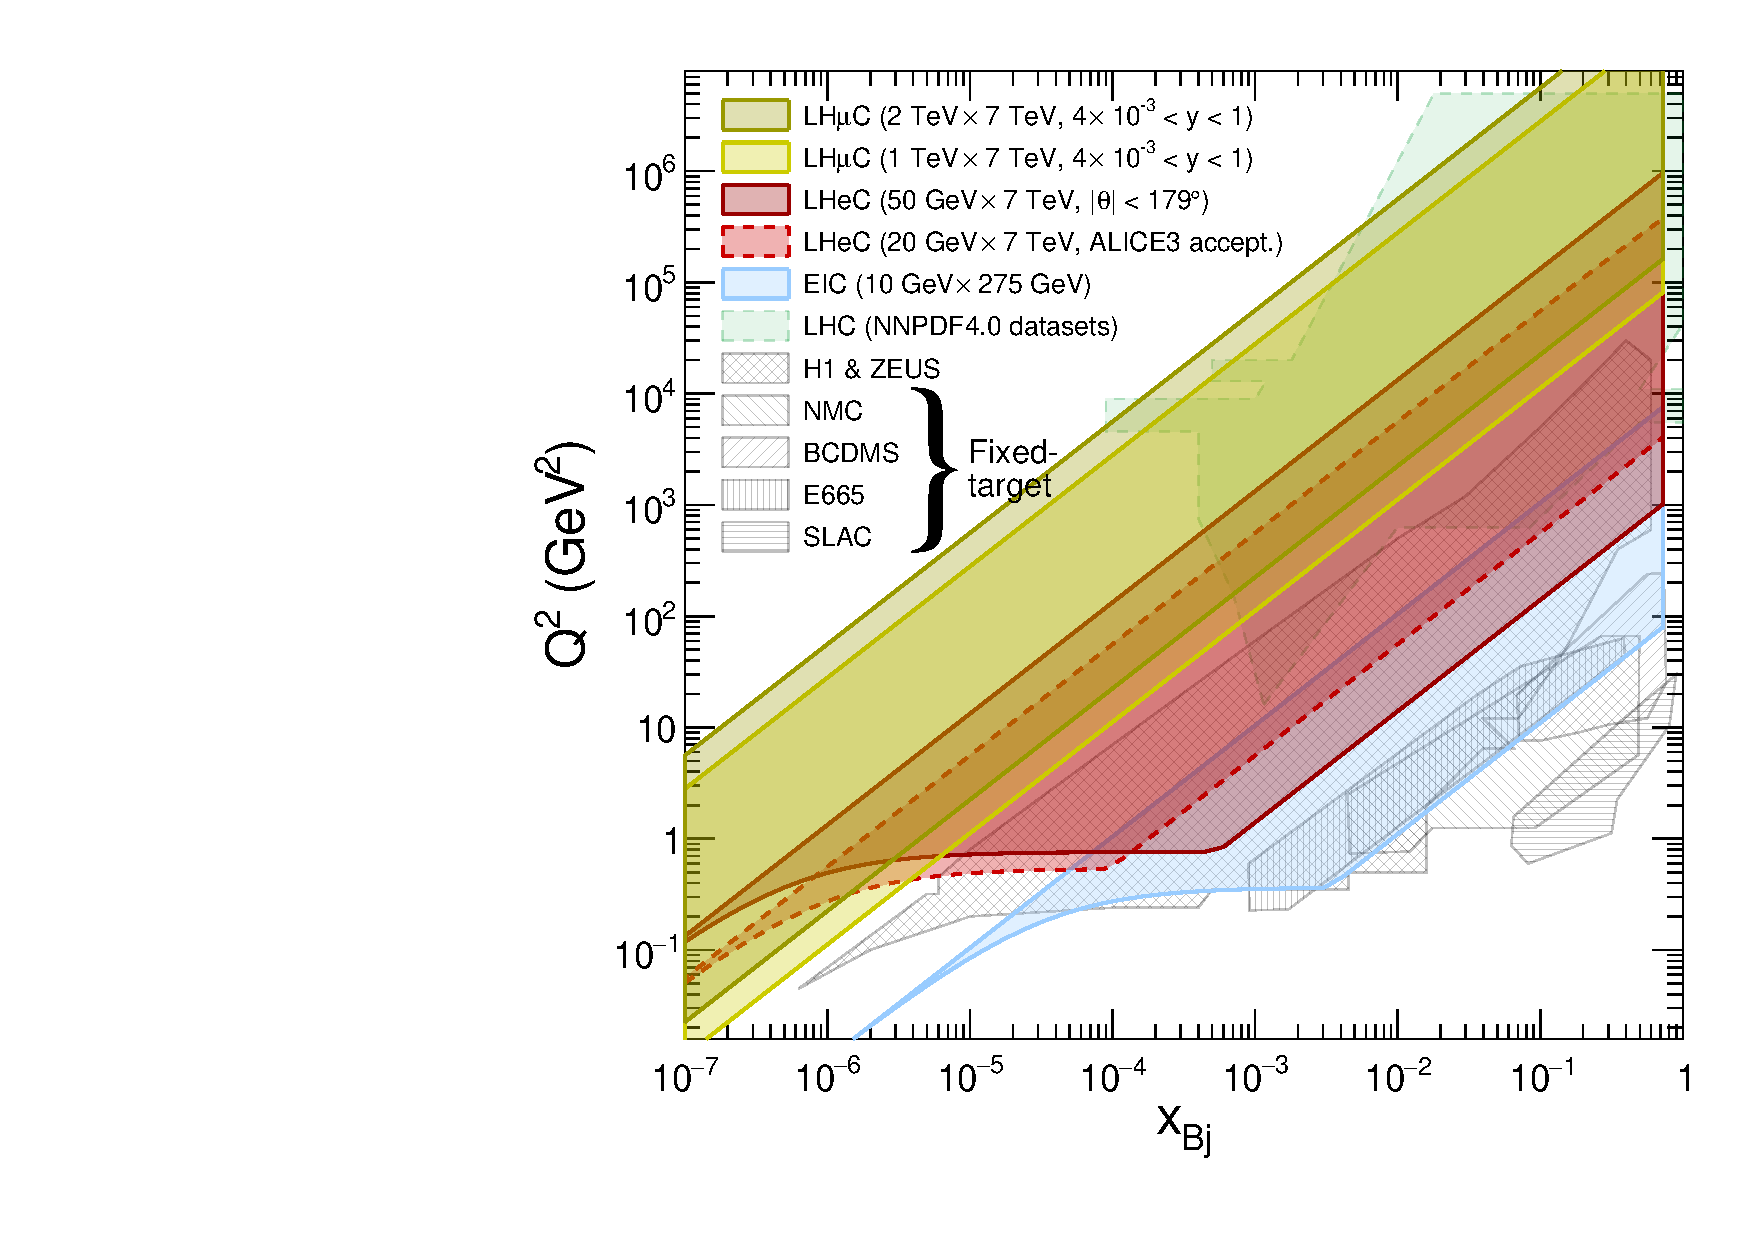
\includegraphics[width=0.50\textwidth]{figures/dis_eta_acceptance.pdf}
\caption{Accessible $(x_{\mathrm{Bj}},Q^2)$ plane from HELP4CERN~\cite{HELP4CERN}, compared with existing 
datasets and planned EIC kinematics. The \lhmuc\ regions use $4\times10^{-3}<y<1$. 
The LHeC curves retain their plotted 20/50~GeV energies and acceptance conventions.} 
\label{fig:coverage}
\end{figure}
%-----------------------------------------




%===============================
\section{Higgs production and precision prospects}\label{sec:higgs}
%===============================


Charged-current (CC) Higgs production proceeds through
$W^+W^-$ fusion. The channel
$\mu^+p\to j\bar\nu_\mu h$ is characterized by an outgoing
quark jet, typically in the forward region, and missing
momentum carried by the antineutrino. A representative
partonic contribution is shown in
Fig.~\ref{fig:higgs-production}(a).
Neutral-current (NC) production,
$\mu^+p\to\mu^+jh$, proceeds through $ZZ$ fusion and retains
the scattered charged lepton, providing a complementary
experimental signature; an example is shown in
Fig.~\ref{fig:higgs-production}(b).


%----------------------------------
\begin{figure}[htbp]
\centering
%---------------- Charged-current production ----------------
\begin{minipage}[t]{0.48\textwidth}
\centering
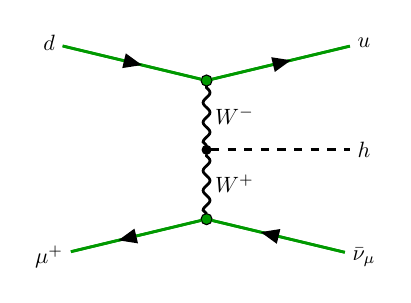
\begin{tikzpicture}[scale=0.80, transform shape]
\begin{feynman}
\vertex (i1) at (-2.5,  1.7) {\(d\)};
\vertex (i2) at (-2.5, -1.7) {\(\mu^{+}\)};
				
\vertex [dot, fill=green!60!black, minimum size=5pt]
(v1) at (0, 1.1) {};
\vertex [dot, fill=green!60!black, minimum size=5pt]
(v2) at (0,-1.1) {};
\vertex [dot, minimum size=4pt]
(m1) at (0,0) {};
				
\vertex (o1) at (2.5,  1.7) {\(u\)};
\vertex (o2) at (2.5, -1.7) {\(\bar{\nu}_{\mu}\)};
\vertex (h1) at (2.5,  0.0) {\(h\)};
				
\diagram*{
(i1) -- [fermion, draw=green!60!black, line width=1pt] (v1)
-- [fermion, draw=green!60!black, line width=1pt] (o1),
(i2) -- [anti fermion, draw=green!60!black, line width=1pt] (v2)
-- [anti fermion, draw=green!60!black, line width=1pt] (o2),
(v1) -- [boson, edge label=\(W^{-}\), line width=1pt] (m1),
(m1) -- [boson, edge label=\(W^{+}\), line width=1pt] (v2),
(m1) -- [scalar, line width=1pt] (h1),
};
\end{feynman}
\end{tikzpicture}
		
\smallskip
{\small (a) Charged-current production}
\end{minipage}
\hfill
%---------------- Neutral-current production ----------------
\begin{minipage}[t]{0.48\textwidth}
\centering
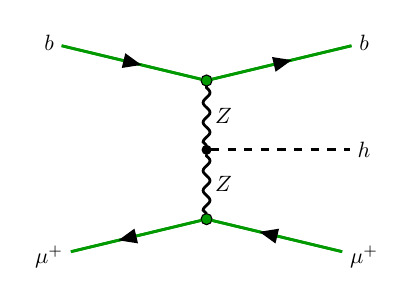
\begin{tikzpicture}[scale=0.80, transform shape]
\begin{feynman}
\vertex (i1) at (-2.5,  1.7) {\(b\)};
\vertex (i2) at (-2.5, -1.7) {\(\mu^{+}\)};
				
\vertex [dot, fill=green!60!black, minimum size=5pt]
(v1) at (0, 1.1) {};
\vertex [dot, fill=green!60!black, minimum size=5pt]
(v2) at (0,-1.1) {};
\vertex [dot, minimum size=4pt]
(m1) at (0,0) {};
				
\vertex (o1) at (2.5,  1.7) {\(b\)};
\vertex (o2) at (2.5, -1.7) {\(\mu^{+}\)};
\vertex (h1) at (2.5,  0.0) {\(h\)};
				
\diagram*{
(i1) -- [fermion, draw=green!60!black, line width=1pt] (v1)
-- [fermion, draw=green!60!black, line width=1pt] (o1),
(i2) -- [anti fermion, draw=green!60!black, line width=1pt] (v2)
-- [anti fermion, draw=green!60!black, line width=1pt] (o2),
(v1) -- [boson, edge label=\(Z\), line width=1pt] (m1),
(m1) -- [boson, edge label=\(Z\), line width=1pt] (v2),
(m1) -- [scalar, line width=1pt] (h1),
};
\end{feynman}
\end{tikzpicture}
		
\smallskip
{\small (b) Neutral-current production}
\end{minipage}

\caption{Representative tree-level diagrams for Higgs production
in positive-muon--proton collisions:
(a) the charged-current subprocess
$\mu^+d\to\bar\nu_\mu uh$ through $W^+W^-$ fusion;
(b) the neutral-current subprocess
$\mu^+b\to\mu^+bh$ through $ZZ$ fusion.
The outgoing
quark contributes to the jet signature. }
\label{fig:higgs-production}
\end{figure}
%----------------------------------

The rates in Table~\ref{tab:rates}, however, establish the production
potential. Extracting Higgs couplings additionally requires
decay information, background control, and explicit
assumptions about the Higgs width.






%===============================
\subsection{A dedicated \texorpdfstring{$h\to b\bar b$}{h to bb} study}
%===============================


Following the approach of Ref.~\cite{Cheung:2021iev}, we study $\mu^+p\to j\bar\nu_\mu h$, $h\to b\bar b$, against 
CC multijet production and weak-boson-fusion $Z\to b\bar b$. We uses an LHeC-like fast detector simulation 
with Delphes~\cite{deFavereau:2013fsa}, a stated 75\% $b$-tagging factor, exactly two selected $b$-jets, 
and $|m_{bb}-m_h|<25~\mathrm{GeV}$. The quoted rate precision includes statistical errors only:

%----------------------------------
\begin{equation}
\frac{\Delta\sigma}{\sigma}=\frac{\sqrt{N_s+N_b}}{N_s},
\label{eq:stat}
\end{equation}
%----------------------------------

where $N_s$ and $N_b$ are the selected signal and background counts. 
The source reports $1.19\%$ and $0.69\%$ for its 500~GeV and 1~TeV muon studies, 
respectively. 
The conversion to a bottom-Yukawa constraint uses external information on $R=g_{hWW}^2/\Gamma_h$, 
where $\Gamma_h$ is the total Higgs width. 
Since the measured production-times-decay rate scales as $R\,g_{hbb}^2$, the source combines 
independent relative uncertainties in quadrature: 

%----------------------------------
\begin{equation}
\frac{\Delta g_{hbb}}{g_{hbb}}
=\frac12\sqrt{\left(\frac{\Delta\sigma}{\sigma}\right)^2+
\left(\frac{\Delta R}{R}\right)^2}.
\label{eq:coupling}
\end{equation}
%----------------------------------

With the external $\Delta R/R=0.985\%$ input following the FCC-ee benchmark treatment of Ref.~\cite{Cheung:2021iev}, 
we obtain coupling precision of $0.77\%$ and $0.60\%$. 




%===============================
\subsection{Exploratory combined coupling fit}\label{subsec:combined-coupling-fit}
%===============================

We perform a complementary combined Higgs-coupling fit in the
$\kappa$-3 framework~\cite{HELP4CERN,deBlas:2019rxi,Armadillo:2026mvp}.
For this exploratory study, the statistical components of the
LHeC signal-strength uncertainties are rescaled using the
Higgs-production rates, while retaining the source assumptions
about backgrounds, acceptance, efficiency, and systematic factors.
The results are expressed in terms of fermion, vector-boson,
and effective loop-induced coupling modifiers, together with
constraints on invisible and undetected Higgs decays.

Figure~\ref{fig:higgs-couplings} summarizes the exploratory
$\kappa$-3 fit~\cite{HELP4CERN,deBlas:2019rxi}, performed with
SMEFiT~\cite{Armadillo:2026mvp} by rescaling the LHeC
signal-strength uncertainties while retaining the source
assumptions about backgrounds, acceptance, efficiency, and
systematic factors. The LHeC+\lhmuc\ combinations are compared
with the LHeC reference and HL-LHC
baselines~\cite{ATLAS:2025eii}; ``HL-LHC improved'' incorporates
reduced PDF and $\alpha_s$
uncertainties~\cite{Ahmadova:2025vzd}. The combined
$\kappa_W$ uncertainties reach $0.28\%$, $0.19\%$, and
$0.16\%$ for the 500~GeV, 1~TeV, and 2~TeV stages,
respectively. At 2~TeV, the reported uncertainties on
$\kappa_b$, $\kappa_c$, $\kappa_g$, and $\kappa_\gamma$
are $0.50\%$, $1.2\%$, $0.75\%$, and $1.1\%$,
whereas the improvements in $\kappa_t$, $\kappa_\mu$,
and $\kappa_{Z\gamma}$ are smaller. Since these measurements
do not independently determine the Higgs width, the fit
imposes $\kappa_V(\kappa_W,\kappa_Z)\le1$, with vector
uncertainties defined as $1-\kappa_V(68\%)$.
These are model-dependent combined projections, distinct
from the dedicated $h\to b\bar b$ extraction and from standalone \lhmuc\ sensitivities.

%----------------------------------
\begin{figure}[tbp]
\centering
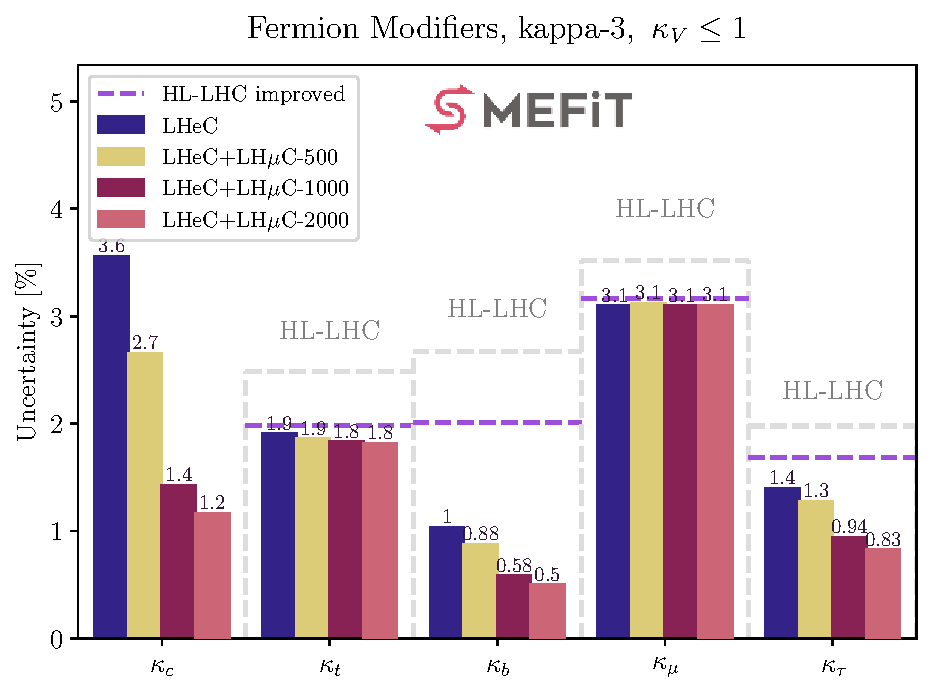
\includegraphics[width=.49\textwidth]{figures/LHmuC_fermion.pdf}
\hfill
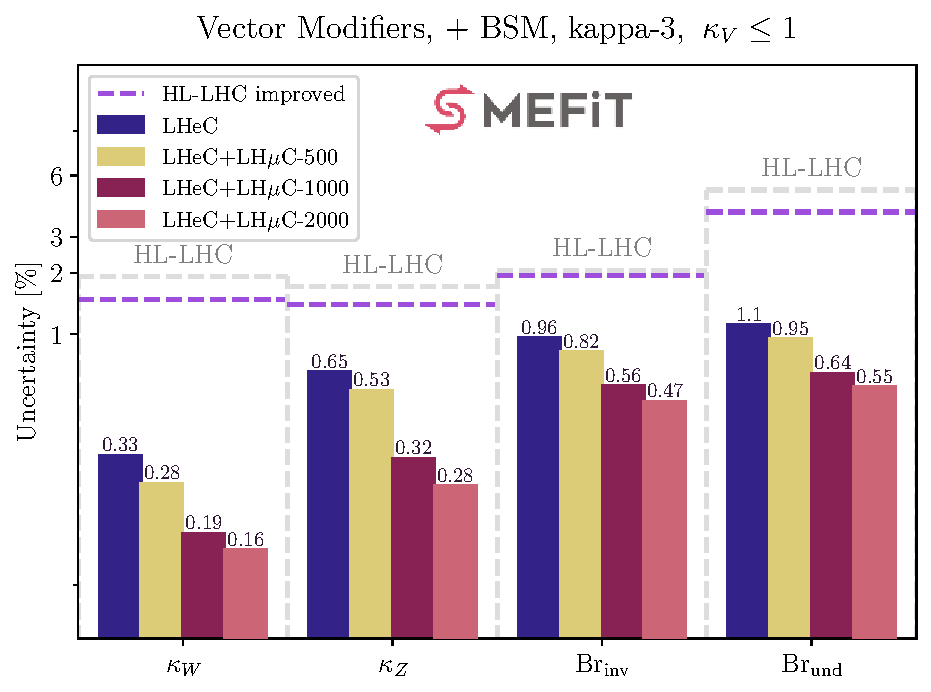
\includegraphics[width=.49\textwidth]{figures/LHmuC_vector.pdf}
\smallskip
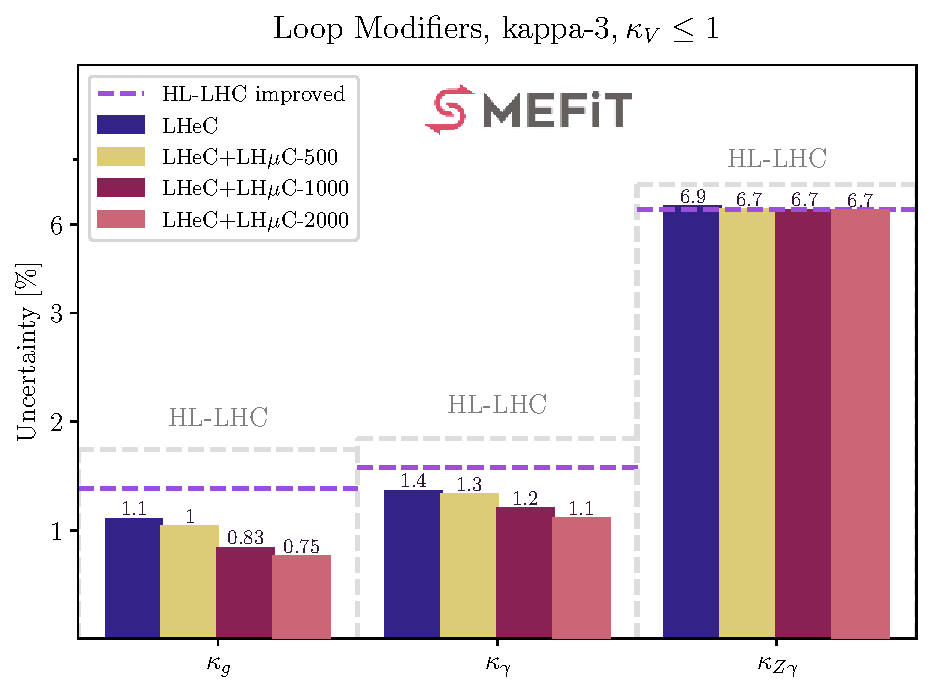
\includegraphics[width=.49\textwidth]{figures/LHmuC_loop.pdf}
\caption{Exploratory $\kappa$-3 fit projections from
HELP4CERN~\cite{HELP4CERN}: fermion modifiers (upper left),
vector modifiers and invisible/undetected branching
fractions (upper right), and effective loop-induced
modifiers (lower). Results are shown for the LHeC and
combined LHeC+\lhmuc\ stages, with HL-LHC baselines.
Coupling uncertainties and branching-fraction constraints
are expressed in percent; the fit assumes $\kappa_V\le1$.}
\label{fig:higgs-couplings}
\end{figure}
%----------------------------------

Taken together, these projections illustrate the complementary
information provided by the different Higgs channels.
The higher-energy combinations improve several fermion,
vector, and loop-induced coupling constraints, although the
size of the improvement varies substantially between
observables. The results remain exploratory combined
projections: they do not represent standalone \lhmuc\
measurements or independent detector-level sensitivity
studies for every channel. Establishing a complete precision
programme requires dedicated analyses of detector response,
backgrounds, systematic uncertainties, and their correlations.





%===============================
\section{Electroweak and top physics}\label{sec:ewtop}
%===============================

The extension of DIS to high momentum transfer provides a complementary 
setting for testing the electroweak 
interaction. NC and CC measurements probe different combinations of quark 
flavours and electroweak couplings, 
while their kinematic dependence can help separate changes in the hard 
interaction from proton-structure effects. 
Weak-mixing-angle studies and constraints on effective interactions are 
therefore motivated by the 
available phase space~\cite{HELP4CERN,LHeC:2020van}. 

In the top sector, CC single-top production gives access to the charged-current interaction 
involving the top quark and motivates studies of the $Wtb$ vertex and CKM parameters. 
NC top-pair production offers a distinct final state and probes the top sector through 
complementary production and decay observables~\cite{HELP4CERN}. 
Table~\ref{tab:rates} displays the source-reported growth of both rates with muon energy. 

Studies of anomalous couplings, flavour-changing neutral currents and rare 
top decays are possible necessarily extensions of 
this programme. They should be formulated through explicit observables and 
signal/background analyses 
rather than by translating inclusive rates directly into limits. The expected 
clean lepton-hadron environment is 
advantageous, and dedicated studies need for tagging, acceptance calibration 
and systematic control. 



%===============================
\section{Photon-induced physics}\label{sec:photon}
%===============================


Photon-induced reactions add a complementary production mechanism~\cite{Budnev:1974de,Forthomme:DIS2024,HELP4CERN}. 
The equivalent-photon approximation (EPA) describes the photon fluxes through an 
effective photon-photon luminosity $S_{\gamma\gamma}(W)$. 
Here $W$ is the photon-pair invariant mass, distinct from $\sqrt{s_{\mu p}}$. 
To calculate the lepton-proton level cross section, the $S_{\gamma\gamma}$ need to 
be convoluted with the relevant subprocess cross-section: 

%----------------------------------
\begin{equation}
\sigma(\mu p\to\mu Xp;W>W_0)
=\int_{W_0}^{W_{\max}} dW\,S_{\gamma\gamma}(W)\,\hat\sigma(\gamma\gamma\to X;W).
\label{eq:epa}
\end{equation}
%----------------------------------

Here $W_{\max}$ is the kinematic endpoint. The discussion here concerns 
elastic proton emission with the 
source photon-virtuality restrictions; it does not imply detector selection 
or proton-tagging efficiency.
Figure~\ref{fig:photon} illustrates the photon luminosity and 
cumulative $\tau$-pair production.

%----------------------------------
\begin{figure}[tbp]
\centering
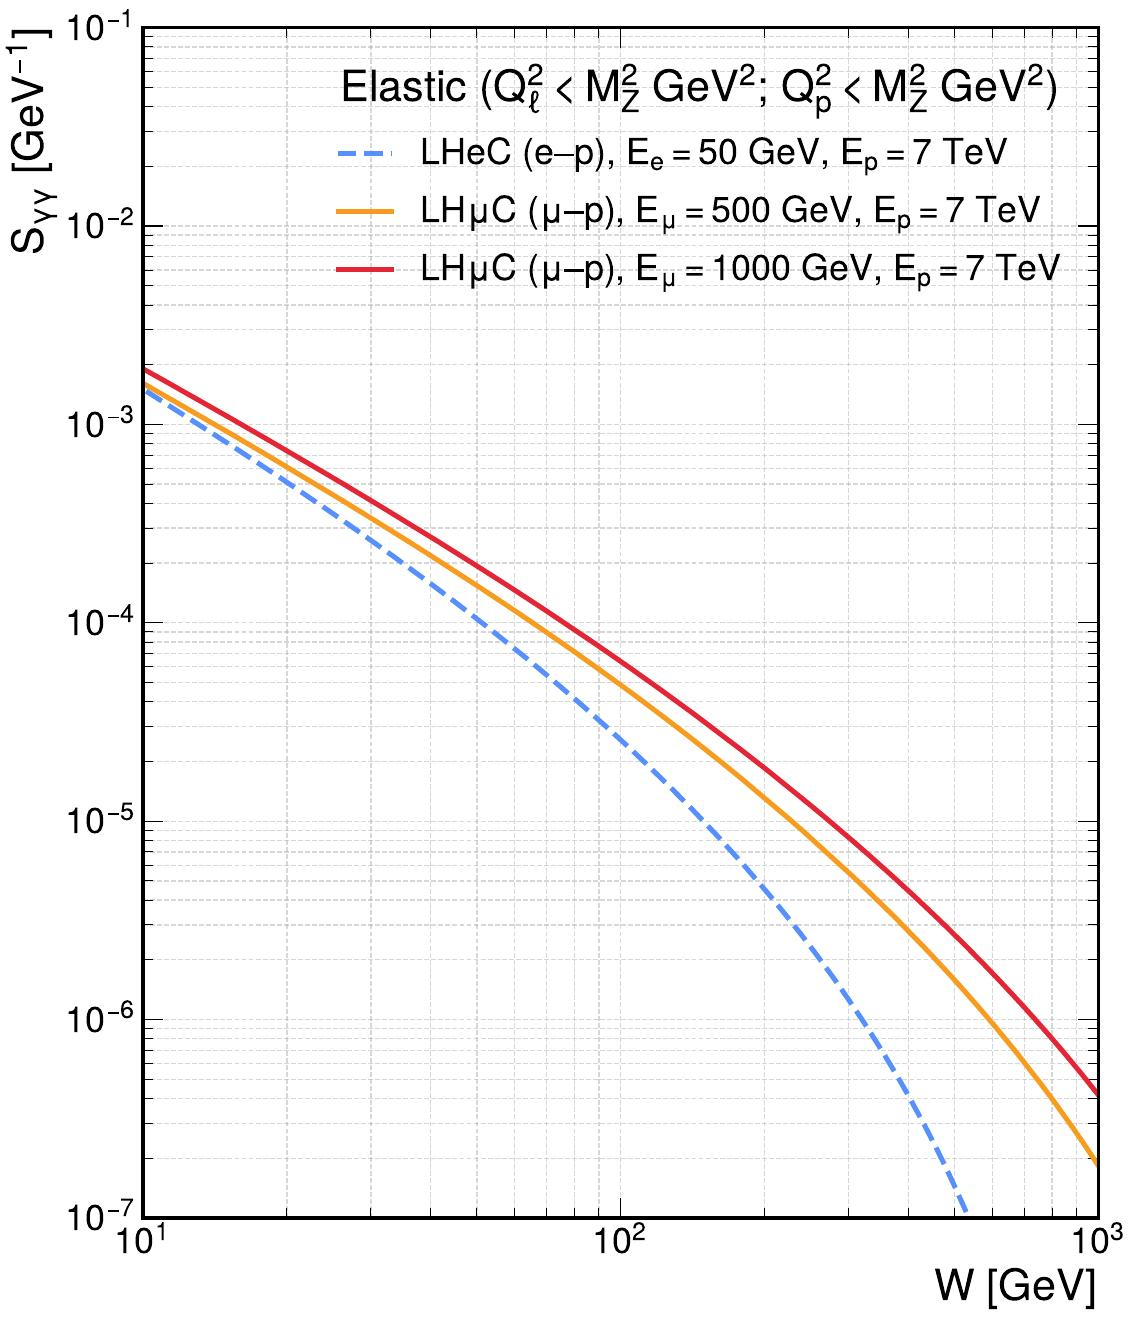
\includegraphics[width=.47\textwidth]{figures/Sgg.jpg}\hfill
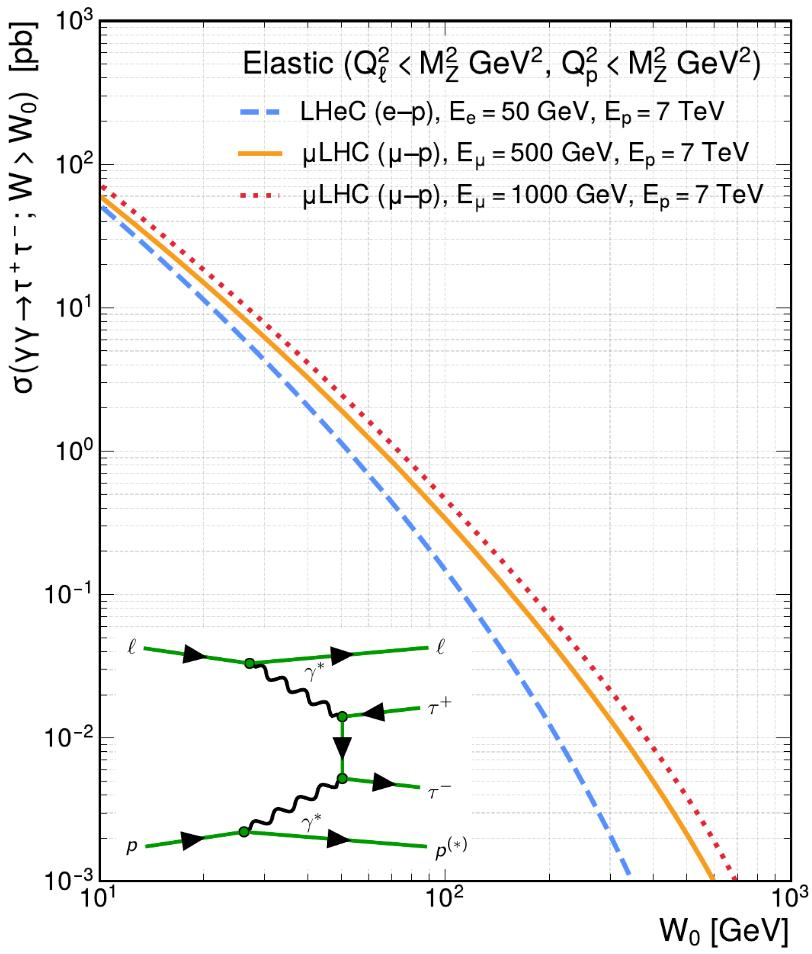
\includegraphics[width=.47\textwidth]{figures/yytautau.jpg}
\caption{Elastic effective photon luminosity (left) and cumulative $\tau$-pair 
	cross-section $\sigma(W>W_0)$ (right). 
The curves compare 50~GeV electrons and 500/1000~GeV muons on 7~TeV protons.}
\label{fig:photon}
\end{figure}
%----------------------------------

For $\tau^+\tau^-$ production above $W_0=10~\mathrm{GeV}$, we calculate the cumulative cross-sections 
of $50.37$, $58.56$ and $70.3$~pb for 50~GeV electrons, 500~GeV muons and 1~TeV muons, 
respectively, on 7~TeV protons~\cite{Khanpour:DIS2026}. 

The enhanced high-mass photon luminosity at \lhmuc\
increases the production rates relative to the LHeC,
with a channel-dependent enhancement. For example,
the quoted elastic $W^+W^-$ cross-sections are approximately
4.5 and 7 times larger for the 500~GeV and 1~TeV muon
options, respectively, than for the 50~GeV LHeC benchmark.
At equal integrated luminosity, these enhancements translate
into larger produced samples; reconstructed yields also
depend on acceptance and selection efficiencies. 
Beyond $\tau^+\tau^-$ and $W^+W^-$, the programme includes
loop-induced $\gamma\gamma\to ZZ$, top-pair production
$\gamma\gamma\to t\bar t$, and pair production of charged
BSM states, including higgsinos and
sleptons~\cite{HELP4CERN,Khanpour:DIS2026}.  
The high-mass tails (as shown in Figure~\ref{fig:photon}) motivate studies of tau 
electromagnetic properties and gauge-boson interactions and 
our anomalous-coupling deformations 
illustrate possible shape sensitivity.  



%===============================
\section{BSM perspectives}\label{sec:BSM}
%===============================


The muon beam also provides access to interactions involving muons and proton constituents. 
Examples in HELP4CERN include resonant squark production 
through an $R$-parity-violating $\mu q$ coupling and 
color-octet muon production through a $\mu g$ interaction~\cite{HELP4CERN,Cheung:2021iev}. 
These mechanisms illustrate the complementarity between 
single production at a muon-hadron collider and 
searches at proton colliders. Their quantitative reach depends on the model couplings, 
compositeness scale where applicable, luminosity and event selection. 




%===============================
\section{Conclusions}\label{sec:outlook}
%===============================


The \lhmuc\ benchmarks combine an enlarged DIS phase space with 
substantial Higgs and top production rates. 
The dedicated $h\to b\bar b$ analysis and exploratory combined fit 
demonstrate why Higgs precision is a 
central motivation, while also showing the importance of external 
width/coupling information and explicit fit assumptions. 
Electroweak, top and photon-induced measurements broaden the programme, 
with muon-coupled BSM channels 
supplying additional discovery opportunities. 
The present projections, however, motivate further work on detector response, 
backgrounds, systematic uncertainties and consistent analysis 
benchmarks before a 
complete experimental sensitivity programme can be established.

\begin{thebibliography}{99}

\bibitem{Akturk:2025ubm}
D.~Akturk et al., \emph{$\mu$LHC: Antimuon Ring and High Luminosity-LHC-Based $\mu^+p$ Collider},
\href{https://doi.org/10.1093/ptep/ptag031}{PTEP \textbf{2026}, 033C04},
\href{https://arxiv.org/abs/2506.15445}{arXiv:2506.15445}.



\bibitem{LHeC:2020van}
P.~Agostini et al. [LHeC and FCC-he Study Group], \emph{The Large Hadron--Electron Collider at the HL-LHC},
\href{https://doi.org/10.1088/1361-6471/abf3ba}{J. Phys. G \textbf{48} (2021) 110501},
\href{https://arxiv.org/abs/2007.14491}{arXiv:2007.14491}.



\bibitem{Ahmadova:2025vzd}
F.~Ahmadova et al., \emph{The Large Hadron electron Collider as a bridge project for CERN},
\href{https://arxiv.org/abs/2503.17727}{arXiv:2503.17727}.



\bibitem{Khanpour:DIS2026}
H.~Khanpour, \emph{Perspectives for HET physics studies at a muon-hadron collider at CERN},
\href{https://agenda.infn.it/event/47074/contributions/289107/}{presentation at DIS2026},
Bologna, 7 May 2026.



\bibitem{HELP4CERN}
HELP4CERN Study Group, \emph{White Paper on High Energy, High Luminosity Lepton-Hadron Colliders at CERN},
supplied working draft, in preparation.



\bibitem{Andre:2025iar}
K.~D.~J.~Andr{\'e}, L.~Forthomme, B.~Holzer and K.~Piotrzkowski,
``An electron--hadron collider at the high-luminosity LHC,''
\href{https://doi.org/10.1088/1367-2630/ae2e31}
{New J. Phys. \textbf{28}, no.~1, 013001 (2026)},
\href{https://arxiv.org/abs/2503.20475}
{arXiv:2503.20475 [hep-ex]}.


\bibitem{Cheung:2021iev}
K.~Cheung and Z.~S.~Wang, \emph{Physics potential of a muon-proton collider},
\href{https://doi.org/10.1103/PhysRevD.103.116009}{Phys. Rev. D \textbf{103} (2021) 116009},
\href{https://arxiv.org/abs/2101.10476}{arXiv:2101.10476}.



\bibitem{deFavereau:2013fsa}
J.~de Favereau et al. [DELPHES 3], \emph{DELPHES 3, A modular framework for fast simulation of a generic collider experiment},
\href{https://doi.org/10.1007/JHEP02(2014)057}{JHEP \textbf{02} (2014) 057},
\href{https://arxiv.org/abs/1307.6346}{arXiv:1307.6346}.




\bibitem{deBlas:2019rxi}
J.~de Blas et al., \emph{Higgs Boson Studies at Future Particle Colliders},
\href{https://doi.org/10.1007/JHEP01(2020)139}{JHEP \textbf{01} (2020) 139},
\href{https://arxiv.org/abs/1905.03764}{arXiv:1905.03764}.




\bibitem{Armadillo:2026mvp}
T.~Armadillo et al., \emph{New Physics Reach through Precision at Future Colliders: a Multi-Pronged Approach},
\href{https://arxiv.org/abs/2604.16596}{arXiv:2604.16596}.



\bibitem{ATLAS:2025eii}
ATLAS and CMS Collaborations, \emph{Highlights of the HL-LHC physics projections by ATLAS and CMS},
\href{https://arxiv.org/abs/2504.00672}{arXiv:2504.00672}.



\bibitem{Budnev:1974de}
V.~M.~Budnev, I.~F.~Ginzburg, G.~V.~Meledin and V.~G.~Serbo,
\emph{The two-photon particle production mechanism. Physical problems. Applications. Equivalent photon approximation},
\href{https://doi.org/10.1016/0370-1573(75)90009-5}{Phys. Rept. \textbf{15} (1975) 181}.



\bibitem{Forthomme:DIS2024}
L.~Forthomme, H.~Khanpour, K.~Piotrzkowski and Y.~Yamazaki,
\emph{High energy $\gamma\gamma$ interactions at the LHeC},
\href{https://doi.org/10.22323/1.469.0269}{PoS(DIS2024)269 (2025)}.



\end{thebibliography}


\end{document}




